\documentclass[aspectratio=169]{beamer}              % only frames

% for themes, etc.
\mode<presentation>
\usetheme{Madrid} 
\usecolortheme{crane}

%\usepackage{times}  % fonts are up to you
% The usual suspects
\usepackage{multirow, booktabs, dcolumn, color, graphicx} % Tables\usepackage{graphicx}
\usepackage{amsmath,amssymb,amsthm}
% Strikethrough text
\usepackage{soul}
% Adjust box to fit tabulars
\usepackage{adjustbox}
% Embed video
\usepackage{media9}
% For notes
\usepackage{pgfpages}
%\setbeameroption{hide notes} % Only slides
%\setbeameroption{show only notes} % Only notes
\setbeameroption{show notes on second screen=right} % Both
% Give a slight yellow tint to the notes page
%\setbeamertemplate{note page}{\pagecolor{yellow!5}\insertnote}\usepackage{palatino}
% Use colors by name
\usepackage{xcolor}
% EMBEDDING VIDEO IS POSSIBLE WITH PDFPC USE PDF PC to present
\usepackage{multimedia}



% The table highlighting for hypothesis discussion.
\usepackage[beamer,customcolors]{hf-tikz}
\usetikzlibrary{calc}

% To use background images
\newenvironment{colorframe}[2][]{%
\setbeamercolor{background canvas}{bg=#1}
\begin{frame}\color{white}}
{\end{frame}}


% To set the hypothesis highlighting boxes red.
\tikzset{hl/.style={
    set fill color=red!80!black!40,
    set border color=red!80!black,
  },
}

% Set Graphics folder
\graphicspath{{./figures/}}


% these will be used later in the title page
\title{Leaving Traces Online}
\subtitle{Using DNSCrypt}
\author{Irfan Kanat}
\institute[CBS]{{Department of Digitization}\\ Copenhagen Business School}
\date{\today}



\begin{document}

% this prints title, author etc. info from above
\begin{frame}

	\titlepage

	\vfill
	{\tiny \centering This work is licensed under a \href{http://creativecommons.org/licenses/by/4.0/}{Creative Commons Attribution 4.0 International License}.}

\end{frame}

\note{In this module we will talk about what kind of traces we leave going about our daily lives and how to minimize this.}

{
\usebackgroundtemplate{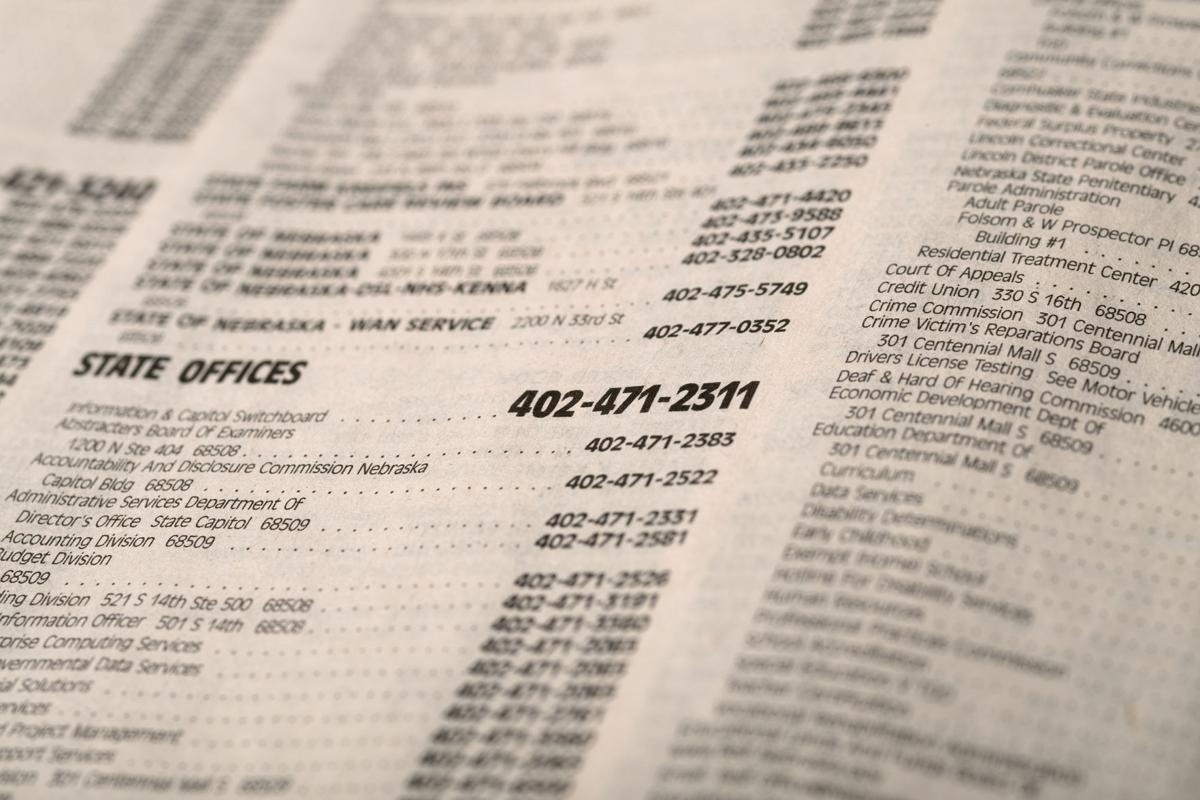
\includegraphics[width=\paperwidth,height=\paperheight]{Phonebook.jpeg}}%
	\begin{frame}
	\frametitle{What is Domain Name System (DNS)}



	\end{frame}
}

\note{
Anytime a piece software on your device tries to connect to a URL, the URL needs to be converted to an address that computer scan understand. This is done through a shared service called Domain Name System.

Think of this as the phone books. In the old days before DNS servers and Internet, when you wanted to call your friend you would look up their name on a phone book.
}


\begin{frame}
	\frametitle{How DNS Works?}

\includegraphics<1>[width = \textwidth, height = .85\textheight, keepaspectratio]{figures/DNS0.png}
\includegraphics<2>[width = \textwidth, height = .85\textheight, keepaspectratio]{figures/DNS1.png}
\includegraphics<3>[width = \textwidth, height = .85\textheight, keepaspectratio]{figures/DNS2.png}
\includegraphics<4>[width = \textwidth, height = .85\textheight, keepaspectratio]{figures/DNS3.png}
\includegraphics<5>[width = \textwidth, height = .85\textheight, keepaspectratio]{figures/DNS4.png}
\includegraphics<6>[width = \textwidth, height = .85\textheight, keepaspectratio]{figures/DNS5.png}

\end{frame}

\note{Almost all software running on your computer needs to make use of the DNS service. Your operating system looking for updates, your browser finding web sites, your cloud file storage syncronizing files... They all will have to use DNS service to look up IP addresses through DNS.

How it works is this way: 

\begin{enumerate}
\item A request is made with a URL (such as reddit.com).
\item Your computer asks the DNS server for the IP address matching the URL.
\item DNS server respons with the IP address.
\item Your computer then rends the request to the correct server.
\item Server responds.
\end{enumerate}
}



\begin{frame}
	\frametitle{What Can Go Wrong}
	\framesubtitle{Snooping}
    
    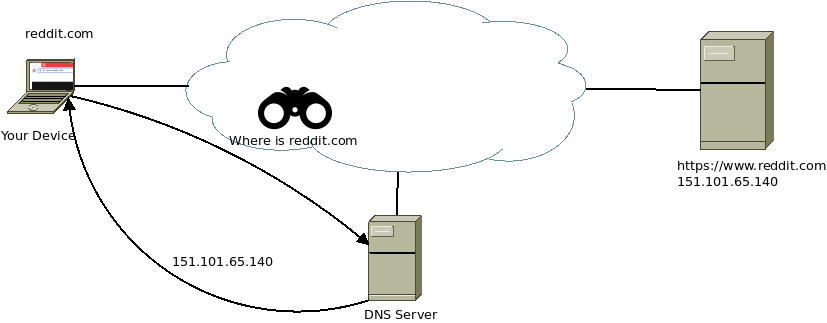
\includegraphics[width = \textwidth, height = .85\textheight, keepaspectratio]{figures/DNSSnoop.png}

\end{frame}

\note{Standard DNS queries are not encrypted. Meaning anyone observing your traffic can easily figure out what you are interested in just by inspecting your DNS querries.}

\begin{frame}
	\frametitle{What Can Go Wrong}
	\framesubtitle{Redirect}
    
	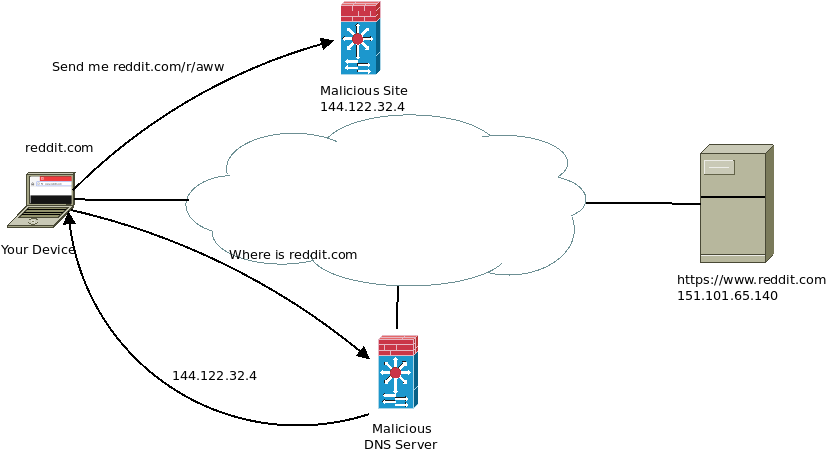
\includegraphics[width = \textwidth, height = .85\textheight, keepaspectratio]{figures/DNS_MIM.png}

\end{frame}

\note{The DNS also does not have authentication mechanisms.

So if the DNS operator acts maliciously, or if someone impersonates your DNS operator, they can redirect you to the wrong addresses.

As an example of this: When you try to reach piracy web sites, the DNS servers redirect you to alternative addresses.

Although not malicious, they redirect you to a site you did not intend to visit.}



\begin{frame}
	\frametitle{What Can Go Wrong}
	\framesubtitle{Denial of Service}    

	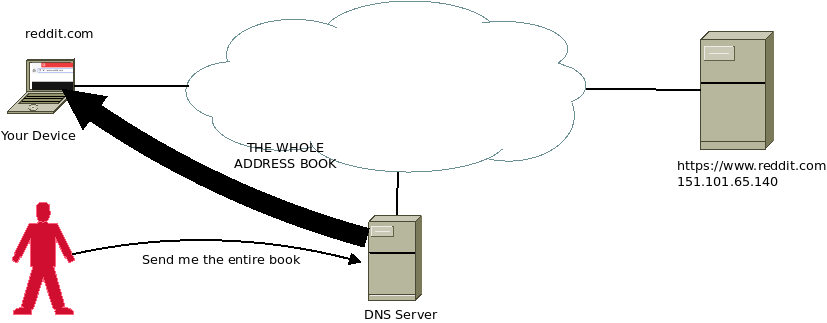
\includegraphics[width = \textwidth, height = .85\textheight, keepaspectratio]{figures/DNS_DOS.png}

\end{frame}

\note{A common type of attack is called a Denial of Service (DOS) attack. The goal here is to send traffic to the victim to cause a sort of ``traffic jam''.

A single attacker is limited by the amount of traffic they can send. If an attacker could multiply the size of the traffic they generate, they can increase the impact of their DOS attack.

A DNS server can serve as that multiplier. The attacker, pretending (IP Spoofing) to be the victim can make fake requests to DNS servers, asking them for the entire DNS registry (which can be sizable). Therefore using the DNS servers to DOS the victim.
}

\begin{frame}
	\frametitle{DNSCrypt}
    
    Authentication \vspace{1em}

    Encryption

\end{frame}

\note{Enter DNSCrypt, an enhancement of the classical DNS protocol.

DNSCrypt supports authentication, thus malicious parties can not impersonate DNS servers. 

All DNS traffic sent this way is also encrypted. Thus not subject to Snooping.}

\end{document}
